\section{Introduction}

Multilingual large language models (LLMs) frequently exhibit \emph{unintended code-switching} - generating tokens in languages other than the target despite explicit monolingual instructions. Ryan et al.~\cite{ryan-etal-2024-unintended} document how LLM alignment procedures can cause models to default to English even when prompted in other languages, while Yoo et al.~\cite{yoo-etal-2024-csrt} demonstrate that code-switching serves as an effective red-teaming vector, bypassing safety filters. In deployed systems, such behavior degrades user trust. For instance, a customer-service chatbot prompted in Spanish may switch to English mid-response, confusing users. Existing solutions require costly fine-tuning or introduce latency via decoding-time interventions.

We propose \textbf{latent space language steering}, a cheap inference-time method that exploits low-dimensional \emph{language directions} in hidden representations. By applying PCA to parallel translations, we identify linear subspaces separating languages while preserving semantics. Steering via simple projection (one dot product and vector subtraction per token) mitigates code-switching with negligible overhead.

\begin{figure}[ht]
  \centering
  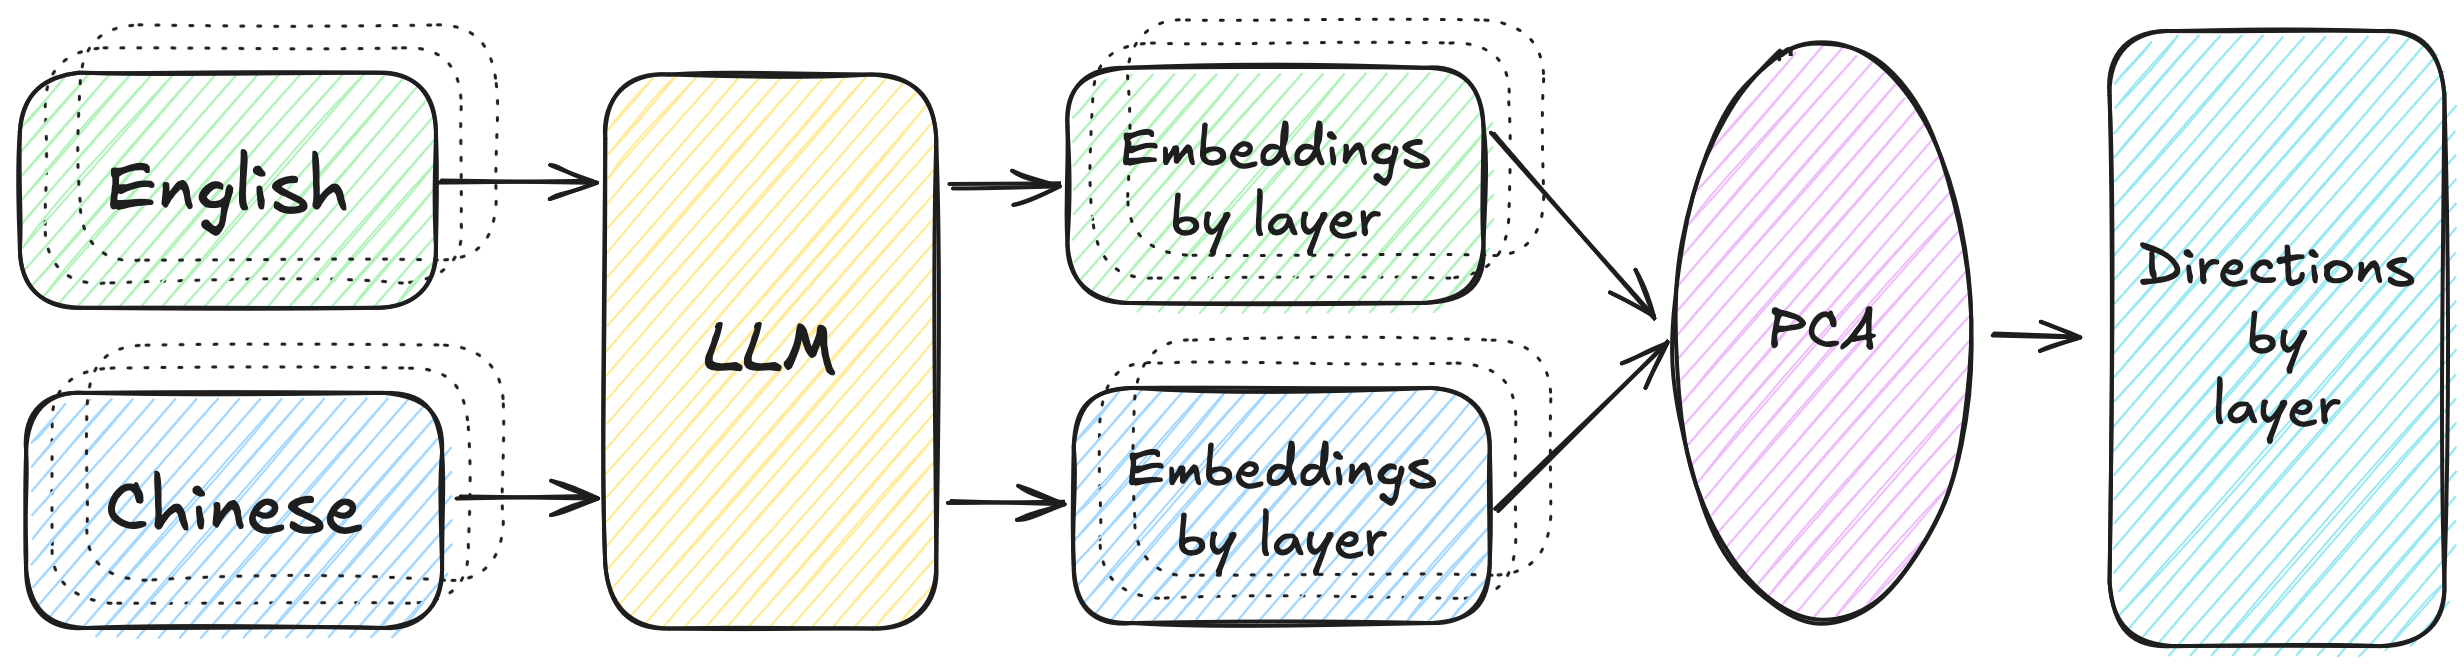
\includegraphics[width=1\linewidth]{images/language_steering_scheme.png}
  \caption{Language steering in hidden space: 1. Collect parallel translations of the same concepts; 2. LLM forward pass to get embeddings by layer; 3. Perform PCA by layer on the merged embeddings.}
  \label{fig:lang_steering_scheme}
\end{figure}

Our analysis shows language identity concentrates in final layers, with PC1 capturing most of the variance and enabling near-perfect language classification. We validate across Qwen2.5 and Llama-3.2 models on multiple language pairs (English, Spanish, Russian, Chinese, and Hindi), demonstrating reduced distributional divergence and substantially lower code-switching rates in generated text.

\paragraph{Contributions.}

\begin{itemize}
  \item We introduce a cheap steering method with negligible overhead requiring only parallel translations for calibration.
  \item Empirically validate across models and language pairs, showing reduced code-switching across both distributional and generation-based evaluations.
  \item Introduce a nearly perfect language classifier based on PCA projections.
  \item Demonstrate language clustering in multilingual LLMs.
  \item Code and data are released to facilitate further research \footnote{\url{https://github.com/fxlrnrpt/language-steering-in-latent-space}}.
\end{itemize}
